\typeout{NT FILE IMPLEM.tex}%
\chapter{Implementation}
\label{cha:implementation}

\begin{quote}
\begin{flushright}
``\emph{Talk is cheap. Show me the code.}'' \\
\textbf{-- Linus Torvalds}, software engineer
\end{flushright}
\end{quote}

This chapter details the implementation of the \gls{uspfs} and \gls{sspfs}
architectures. We begin with a brief overview of the implementation workflow.
Next, we present the base system -- hardware and software components shared by both
architectures -- along with initial validation of the \gls{uav} assembly and its
configuration. We then describe the \gls{uspfs} implementation, deploying the
flight-control and companion stacks on a custom, embedded Linux–based \gls{os}.
Finally, we detail the \gls{sspfs} implementation: each stack is deployed in a
separate \gls{vm} under the Bao hypervisor, and we implement the mailbox
supervisor to coordinate safe access to shared firmware services. The complete
source code is documented in the associated repository~\cite{thesis-sw-github}.

\section{Workflow}
\label{sec:workflow}
Fig.~\ref{fig:uav-main-Implem-Workflow} illustrates the overall implementation
workflow. The \gls{uspfs} path comprises the \emph{Guests}, \emph{Firmware}, and
\emph{Deployment} stages, while the \gls{sspfs} path adds a \emph{Hypervisor}
stage. The workflow has four primary stages:
(1) build guests;
(2) build hypervisor and VMs (for \gls{sspfs} only);
(3) build firmware; and
(4) deployment.
Here, ``guest'' means either a true virtual machine under the Bao hypervisor
(\gls{sspfs}) or a native binary on the \gls{uavic} platform (\gls{uspfs}).

\begin{figure}[!hbt]
  \centering
  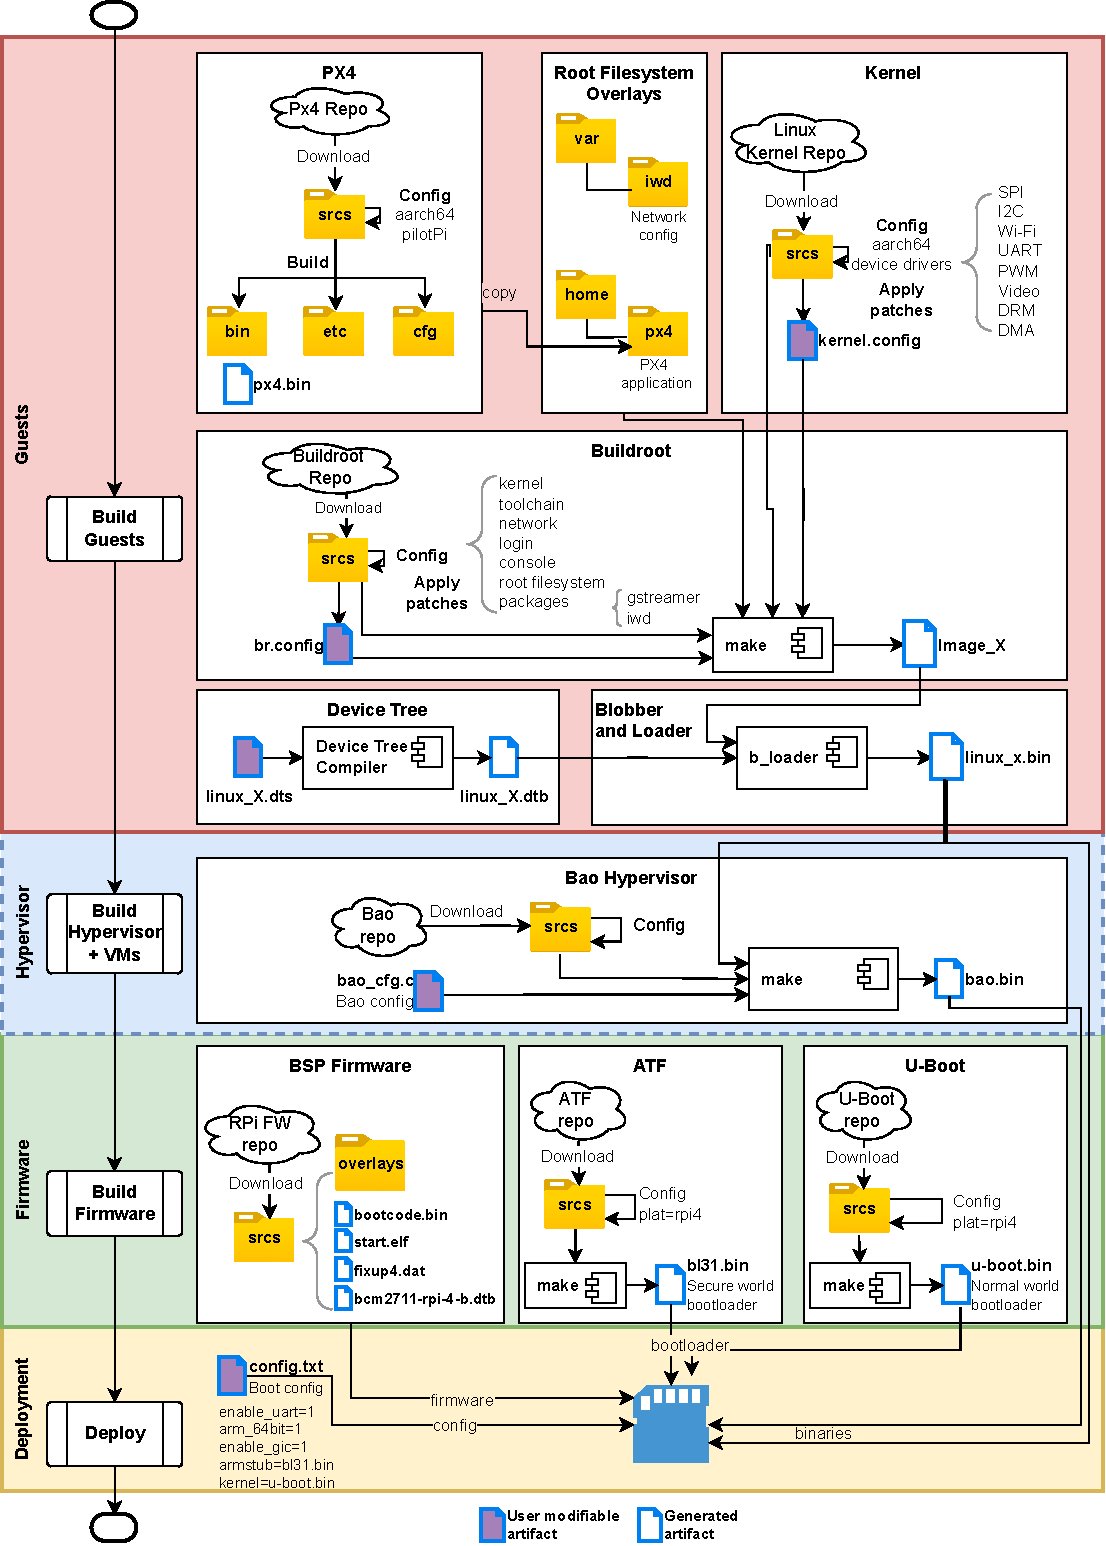
\includegraphics[width=1.0\textwidth]{./img/pdf/uav-main-Implem-Workflow}
  \caption{Implementation workflow}%
  \label{fig:uav-main-Implem-Workflow}
\end{figure}

% \paragraph{Guest construction.}
We first build the guests and their components. In \gls{uspfs}, a single binary
wraps the PX4 and video-surveillance functionality. In \gls{sspfs}, PX4 and the
video pipeline execute concurrently, each in its own isolated guest.
%
The PX4 build targets the \lstinline{PilotPi} board for \lstinline{aarch64},
producing PX4 binaries and runtime configuration files. These, along with network
settings, are staged into Buildroot’s root filesystem for inclusion in the guest
image.
%
The Linux kernel is configured with essential drivers (\gls{spi}, \gls{i2c},
Wi-Fi, video, etc.). Userspace includes network, login, console, and packages
(e.g., \lstinline{gstreamer} for video, \lstinline{iwd} for wireless). Buildroot
then produces a Linux kernel image \lstinline{Image_X} (where \emph{X} denotes
the guest index). A guest-specific device-tree source
\lstinline{linux_X.dts} is compiled to \lstinline{linux_X.dtb}. The
\lstinline{b_loader} tool combines the kernel and DTB into a self-contained
executable with minimal runtime dependencies.
%
For \gls{uspfs}, this yields a single target binary. For \gls{sspfs}, the process
is repeated per guest, producing two binaries later merged by Bao.

% \paragraph{Hypervisor configuration (\gls{sspfs}).}
The \lstinline{bao_cfg.c} file specifies guest paths, entry points, CPU
allocation, memory regions, and device memory/interrupt mappings. Building Bao
produces a consolidated image \lstinline{bao.bin} that encapsulates the
hypervisor plus both guests.
%
% \paragraph{Firmware build.}
We next build the platform firmware. After fetching the Raspberry Pi 4 \gls{bsp},
we configure and build Arm Trusted Firmware (\lstinline{bl31.bin}), required by
Bao, followed by the normal-world bootloader (\lstinline{u-boot.bin}). U-Boot is
responsible for loading the target: \lstinline{linux_X.bin} for \gls{uspfs} or
\lstinline{bao.bin} for \gls{sspfs}.
%
%\paragraph{Deployment.}
Deployment places the boot artifacts onto the \gls{sd} card: Raspberry Pi
firmware, secondary bootloaders, the target binary (\lstinline{linux_X.bin} or
\lstinline{bao.bin}), and \lstinline{config.txt}.

To ensure a correct boot, we follow the \gls{uavic} boot flow in
Fig.~\ref{fig:uav-main-rpi4-boot}. The first-stage bootloader
(\lstinline{bootcode.bin}) initializes hardware, loads firmware from the
\gls{sd} card into \gls{ram}, and parses \lstinline{config.txt}. The GPU
firmware \lstinline{start4.elf} processes \lstinline{config.txt}, enables
\gls{uart} and the \gls{gic}, and transfers control to \lstinline{bl31.bin}
(secure services). Then \lstinline{u-boot.bin} initializes peripherals (including
the console) using the firmware’s \gls{dtb} and its environment, and loads the
target binary. We focus on the more generic \gls{sspfs} case.

When \lstinline{bao.bin} executes, it:
(1) initializes CPUs, memory, and the system console;
(2) configures the interrupt controller;
(3) initializes the mailbox supervisor; and
(4) starts the VM manager.
Each guest then:
(1) boots its Linux kernel using the embedded \gls{dtb};
(2) initializes guest-specific hardware;
(3) mounts the root filesystem; and
(4) launches \lstinline{init}.
The result is isolated guest execution under Bao's supervision.

\begin{figure}[!hbt]
  \centering
  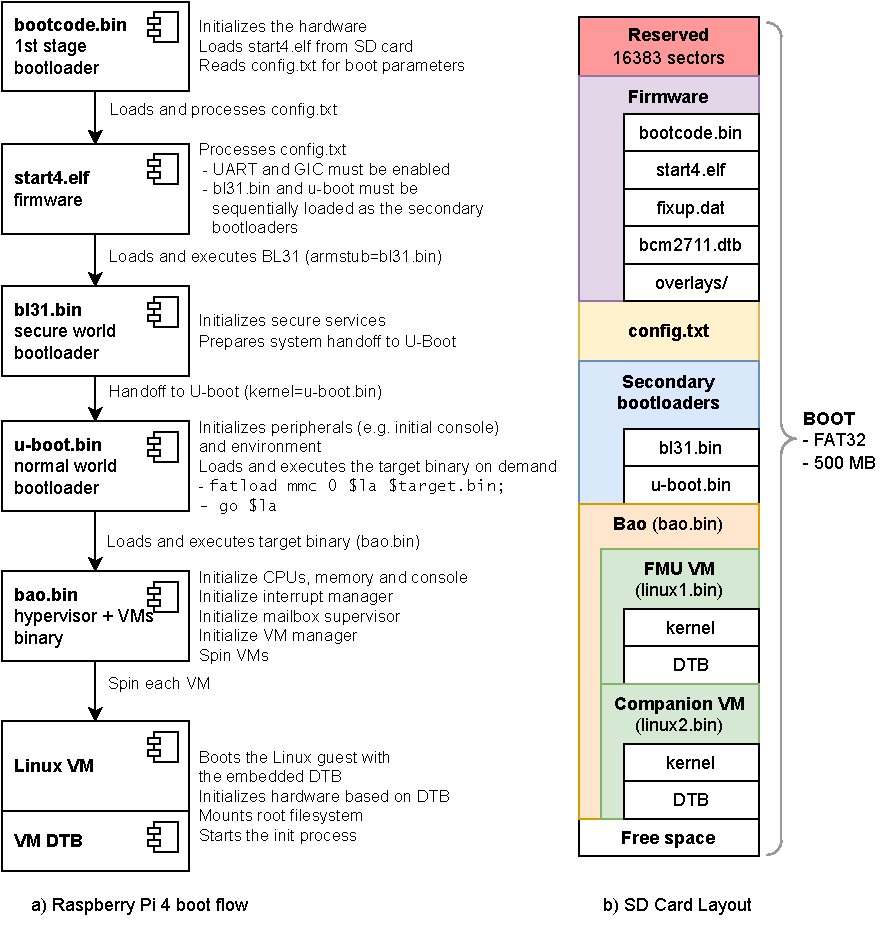
\includegraphics[width=0.9\textwidth]{./img/pdf/uav-main-rpi4-boot}
  \caption{UAVIC boot: (a) platform boot flow; (b) SD card layout}%
  \label{fig:uav-main-rpi4-boot}
\end{figure}

\section{Base system}
\label{sec:base-system}
The base system is the common hardware/software foundation for both \gls{uspfs}
and \gls{sspfs}. It covers \gls{uav} assembly and configuration, plus
stand-alone testing of PX4 and the video-surveillance stack.

\subsection{UAV assembly}
\label{sec:uav-assembly}
The first step is assembling the airframe and configuring it via the \gls{gcs}.
Fig.~\ref{fig:uav-assembly} shows the HoverGames-based build alongside the
QGroundControl interface.

We began with the S500 frame \emph{(3)} as the structural base, then mounted the
landing gear, arms, and electronics plates. The NEO-M8N \gls{gps} module
\emph{(1)} was chosen for cost/performance in urban settings~\cite{gps-neom8n-product}.
Four brushless \gls{dc} motors \emph{(2)} were installed at the arm tips and
driven by opto-coupled 40~A \glspl{esc}.

Power is provided by a 3S \gls{lipo} battery \emph{(12)} (5000~mAh) with an
XT-60 connector \emph{(4)}~\cite{lipo-3s-uav}, yielding roughly 30~minutes at
full throttle (indicative). The \gls{uavic} platform \emph{(7)} combines a
Raspberry~Pi~4 with the PilotPi shield. Telemetry radios \emph{(5)}, \emph{(6)}
link the \gls{uav} to QGroundControl on the \gls{gcs} \emph{(11)}. For early
bring-up we enabled a debug \gls{uart} port \emph{(8)} (omitted in the final
system). The Wi-Fi dongle \emph{(9)} and camera \emph{(10)} required for video
surveillance connect via \gls{usb} to the \gls{uavic}.

Before parameter configuration in QGroundControl, PX4 must be deployed to the
\gls{uavic}. Once PX4 is running, the airframe can be configured over telemetry
radio or Wi-Fi.

\begin{figure}[!hbt]
  \centering
  \includegraphics[width=0.8\textwidth]{./img/png/uav-assembly-annot-final}
  \caption[UAV assembly and configuration]{UAV assembly and configuration: UAV
    (left); Ground Station running QGroundControl (right)}%
  \label{fig:uav-assembly}
\end{figure}

\subsection{PX4}
\label{sec:px4}
After validating the assembly, we deployed PX4 on a general-purpose Linux
\gls{os} on the \gls{uavic} platform. The build procedure is scripted in
\lstinline{src/buildPilot.sh} (see~\cite{thesis-sw-github}) and uses a Python
virtual environment for dependencies. We fetched the PX4 source (including
NuttX applications via submodules), configured the PilotPi target, compiled the
autopilot, and finally deployed the resulting artifacts to the \gls{uavic} over
Wi-Fi.
%
The NuttX \gls{rtos} is configured via the \lstinline{kconfig} system,
analogous to Linux. Listing~\ref{lst:cfg-pilotpi} shows an excerpt of the
configuration (\lstinline{configs/px4/px4.config} in the repo~\cite{thesis-sw-github})
that selects the platform/architecture, toolchain, and the modules/drivers
required for this work.

\begin{longlisting}
\centering
\inputminted[]{kconfig}{./listing/px4.config}
\caption{PX4 configuration file (excerpt)}
\label{lst:cfg-pilotpi}
\end{longlisting}

At startup, PX4 runs \lstinline{pilotpi_mc.config}
(\lstinline{configs/px4/pilotpi_mc.config} in the repo~\cite{thesis-sw-github})
to configure the vehicle and enable services:
\begin{enumerate}[noitemsep,topsep=0pt]
\item Import saved \gls{uav} parameters
\item Select vehicle type and airframe
\item Configure camera triggering via MAVLink
\item Initialize geofence, \gls{cpu} monitoring, and battery status
\item Initialize sensors and actuators
\item Launch the \gls{rc} communication manager
\item Start the main \gls{fmu} state machine
\item Initialize multicopter tasks: navigation, position/attitude control, logging, etc.
\item Enable MAVLink telemetry over radio and Wi-Fi
\item Notify the \gls{gcs} that boot is complete (further configuration by the user)
\end{enumerate}

Fig.~\ref{fig:uav-cfg-px4-boot} shows a successful PX4 initialization: sensors
and actuators are online, and the Wi-Fi link is active
(\lstinline{partner IP: 192.168.1.37}) for MAVLink communication with the \gls{gcs}.
  
\begin{figure}[!hbt]
  \centering
  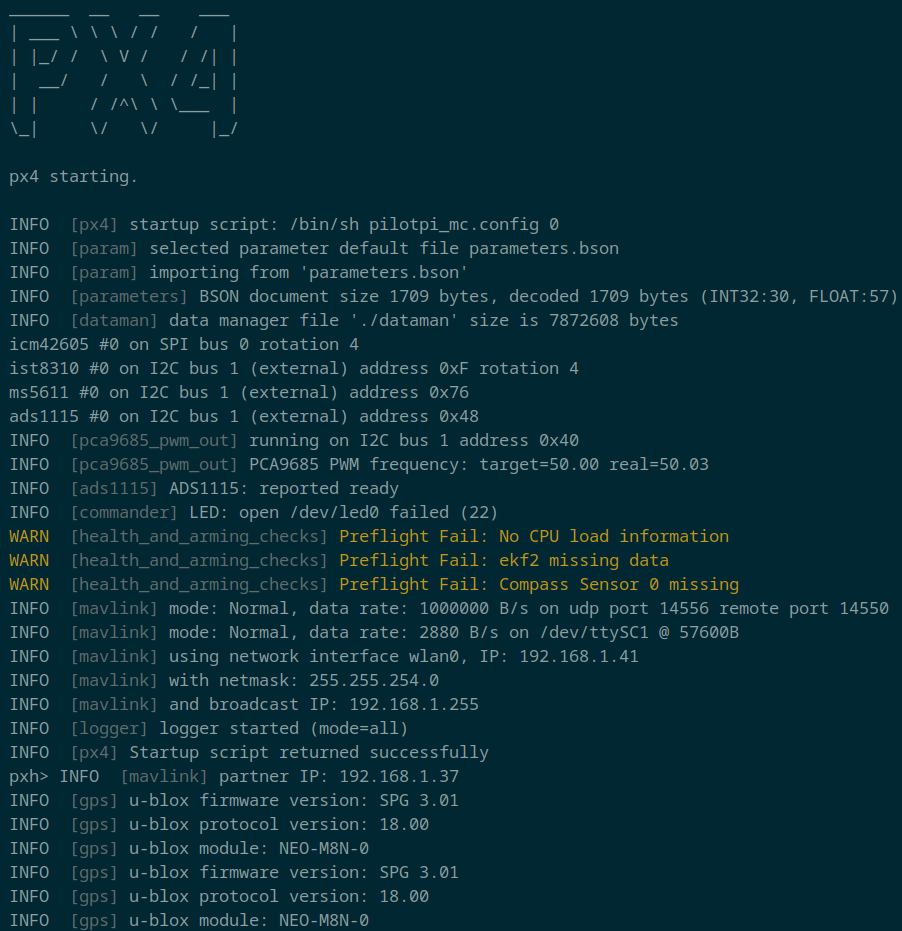
\includegraphics[width=0.6\textwidth]{./img/png/px4-boot}
  \caption{UAV configuration: PX4 boot}
  \label{fig:uav-cfg-px4-boot}
\end{figure}

\subsection{UAV configuration}
\label{sec:uav-configuration}
After pairing the \gls{uav} with the \gls{gcs}, we configured the vehicle in \emph{QGroundControl}.
First, we selected the airframe: the quadrotor NXP HoverGames variant
(Fig.~\ref{fig:uav-cfg-airframe}). Next, we calibrated the compass,
gyroscope, and accelerometer by following the \gls{gcs} prompts and moving the
airframe through the prescribed orientations (Fig.~\ref{fig:uav-cfg-sensors}).
We then configured the power source (battery chemistry/cell count) to obtain
correct power/voltage readings and calibrated \gls{esc} \gls{pwm} minimum and
maximum values to avoid output saturation.

Motor setup followed: we specified motor count and geometry (position/direction),
mapped motors to output channels, and verified spin direction and speed using the
motor test utility. Finally, we reviewed and saved the parameter set; the
resulting configuration can be replicated across PX4 instances to bootstrap
identical \glspl{uav}. Fig.~\ref{fig:uav-cfg-summary} summarizes the final setup.

\begin{figure}[!hbt]
  \centering
  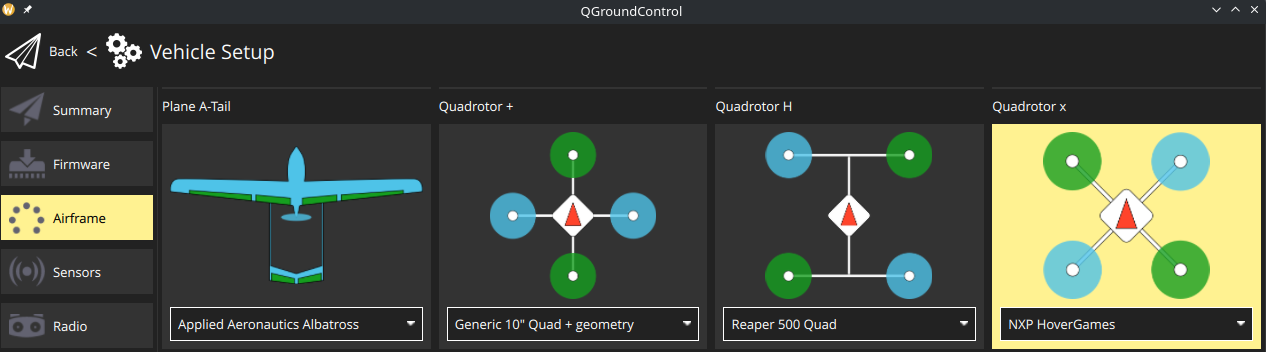
\includegraphics[width=0.9\textwidth]{./img/png/qgc-airframe}
  \caption{UAV configuration: airframe}
  \label{fig:uav-cfg-airframe}
\end{figure}

\begin{figure}[!hbt]
  \centering
  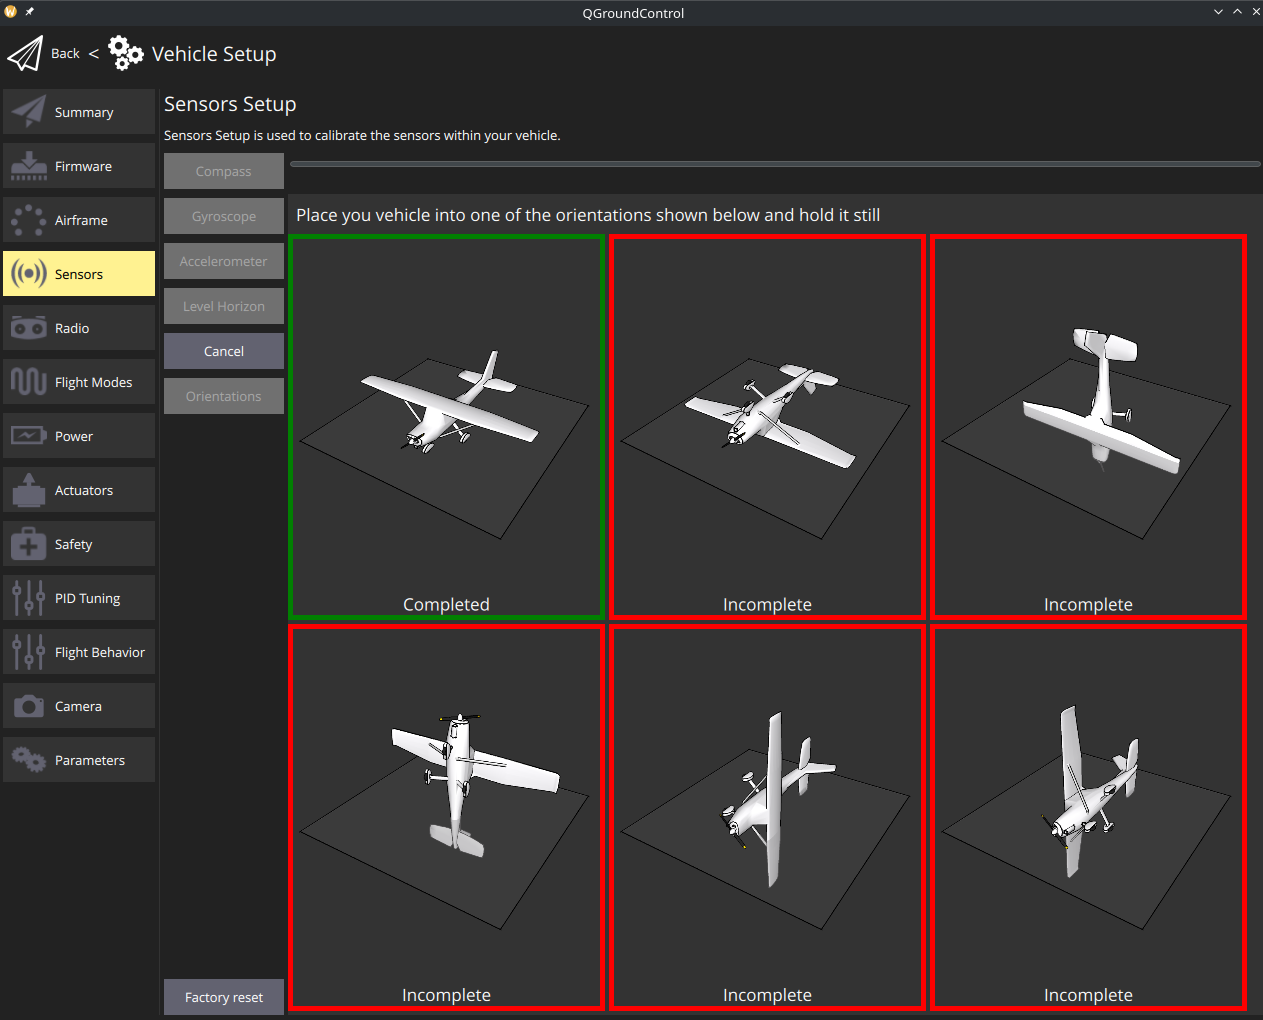
\includegraphics[width=0.9\textwidth]{./img/png/qgc-sensors}
  \caption{UAV configuration: sensor calibration}
  \label{fig:uav-cfg-sensors}
\end{figure}

\begin{figure}[!hbt]
  \centering
  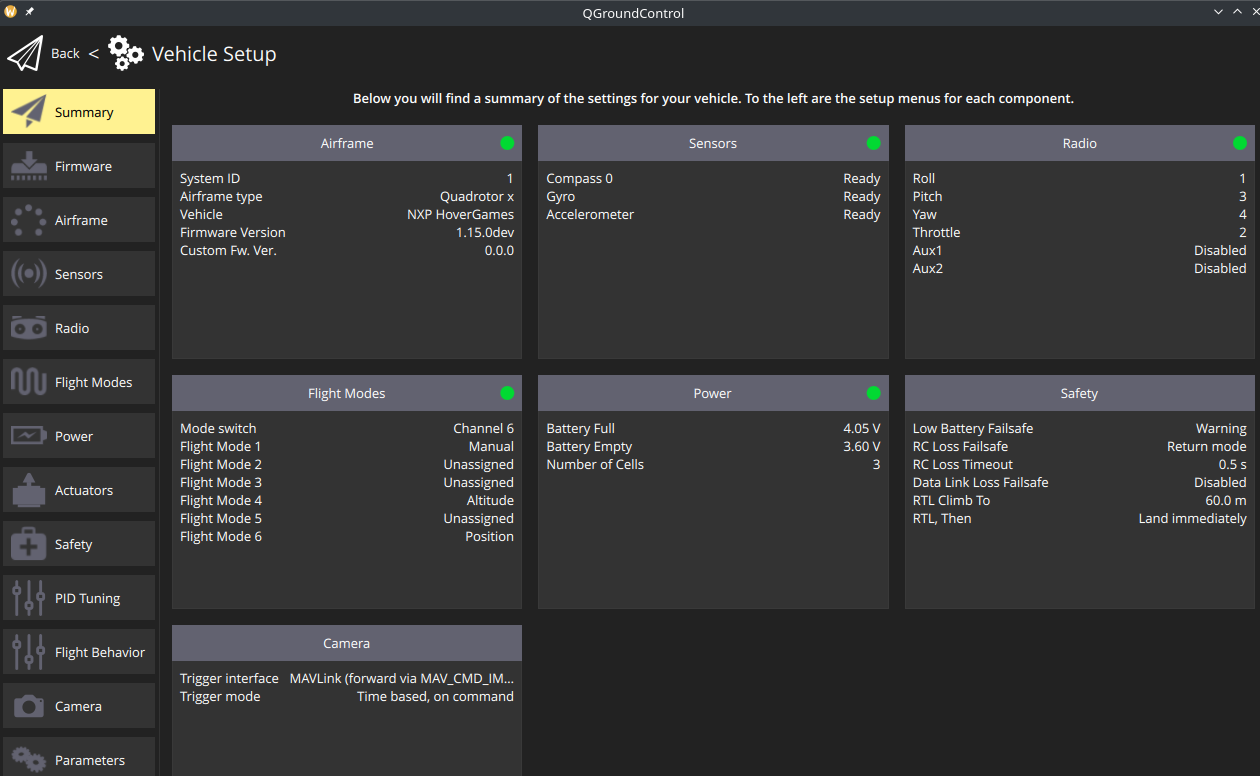
\includegraphics[width=0.92\textwidth]{./img/png/qgc-summary}
  \caption{UAV configuration: summary}
  \label{fig:uav-cfg-summary}
\end{figure}

\subsection{Video surveillance}
\label{sec:video-surveillance}
The video-surveillance pipeline (cf.\ Fig.~\ref{fig:uav-design-unsup}) was
implemented with \lstinline{GStreamer}. Its modular design, broad codec support,
and built-in networking made it easy to iterate and test.
In the sender pipeline, the \gls{uav} captures frames from a USB camera (MJPEG at
640{\(\times\)}480, 30~\gls{fps}), decodes them, re-encodes as H.264, and packets the stream as
RTP over UDP for low-latency delivery. Listing~\ref{lst:gstreamer-sender} shows
the test script, including device selection and the target host/port so only the
designated \gls{gcs} receives the stream.

\begin{longlisting}
\centering
\inputminted[]{bash}{./listing/gstreamerSender.sh}
\caption{Video surveillance sender script}
\label{lst:gstreamer-sender}
\end{longlisting}

In the receiver end, the ground station listens on the chosen UDP port,
unpacks the payload and decodes H.264, converts to a display format, and renders the video.
Listing~\ref{lst:gstreamer-receiver} shows the matching receiver.

\begin{longlisting}
\centering
\inputminted[]{bash}{./listing/gstreamerReceiver.sh}
\caption{Video surveillance receiver script}
\label{lst:gstreamer-receiver}
\end{longlisting}

We validated the end-to-end path by running (1) PX4 (Fig.~\ref{fig:px4-qgc-cam-2})
and the sender on the \gls{uavic} (Fig.~\ref{fig:px4-qgc-cam-3}, top), and
(2) the receiver plus QGroundControl on the \gls{gcs}
(Fig.~\ref{fig:px4-qgc-cam-3}, bottom). As shown in
Fig.~\ref{fig:px4-qgc-cam-1}, telemetry appears in QGroundControl alongside the
live video, validating the pipeline.

\begin{figure}[htb!]
  \centering
  %
  \begin{subfigure}[t]{.48\textwidth}
    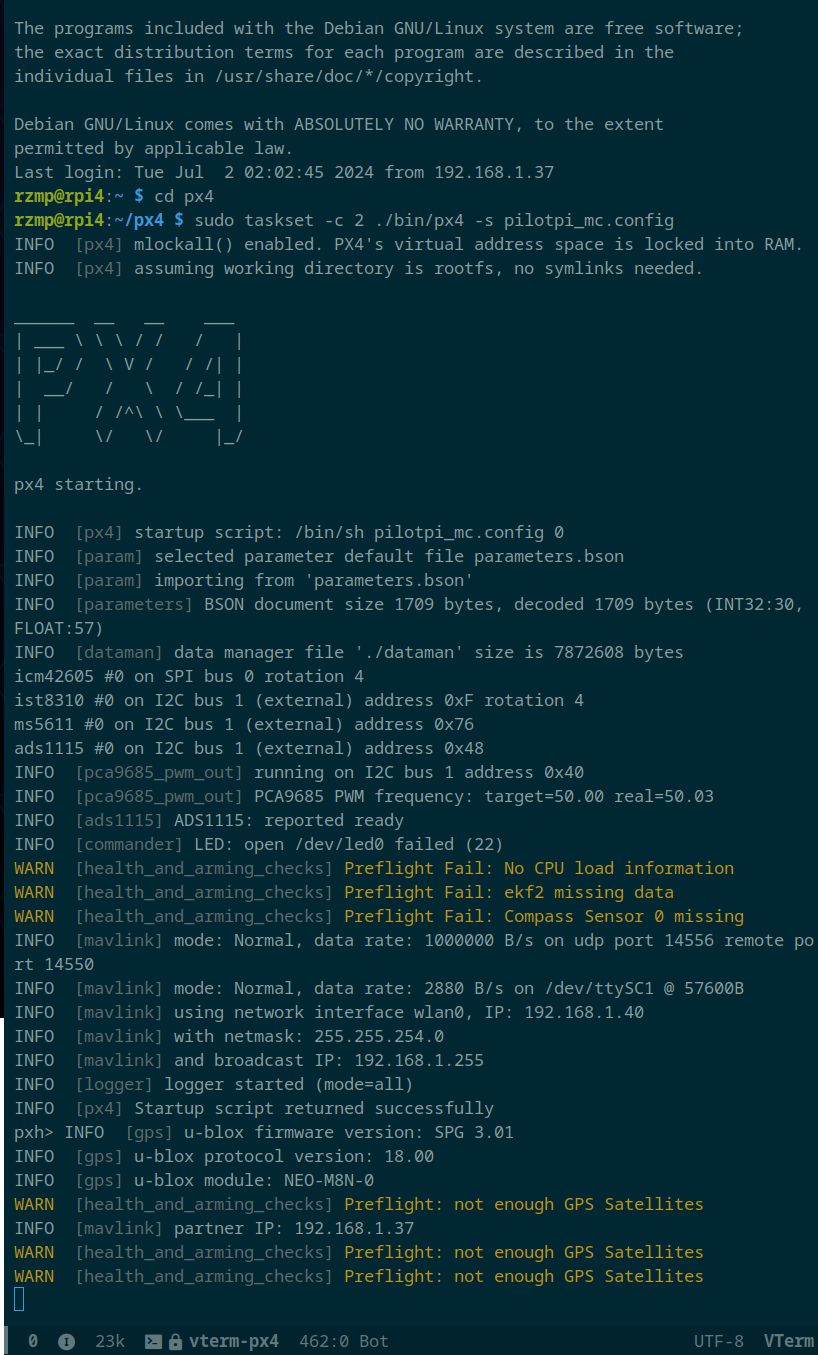
\includegraphics[width=0.89\textwidth]{./img/png/px4-qgc-cam-2}
    \caption{PX4 boot}%
    \label{fig:px4-qgc-cam-2}
  \end{subfigure}
  \begin{subfigure}[t]{.48\textwidth}
    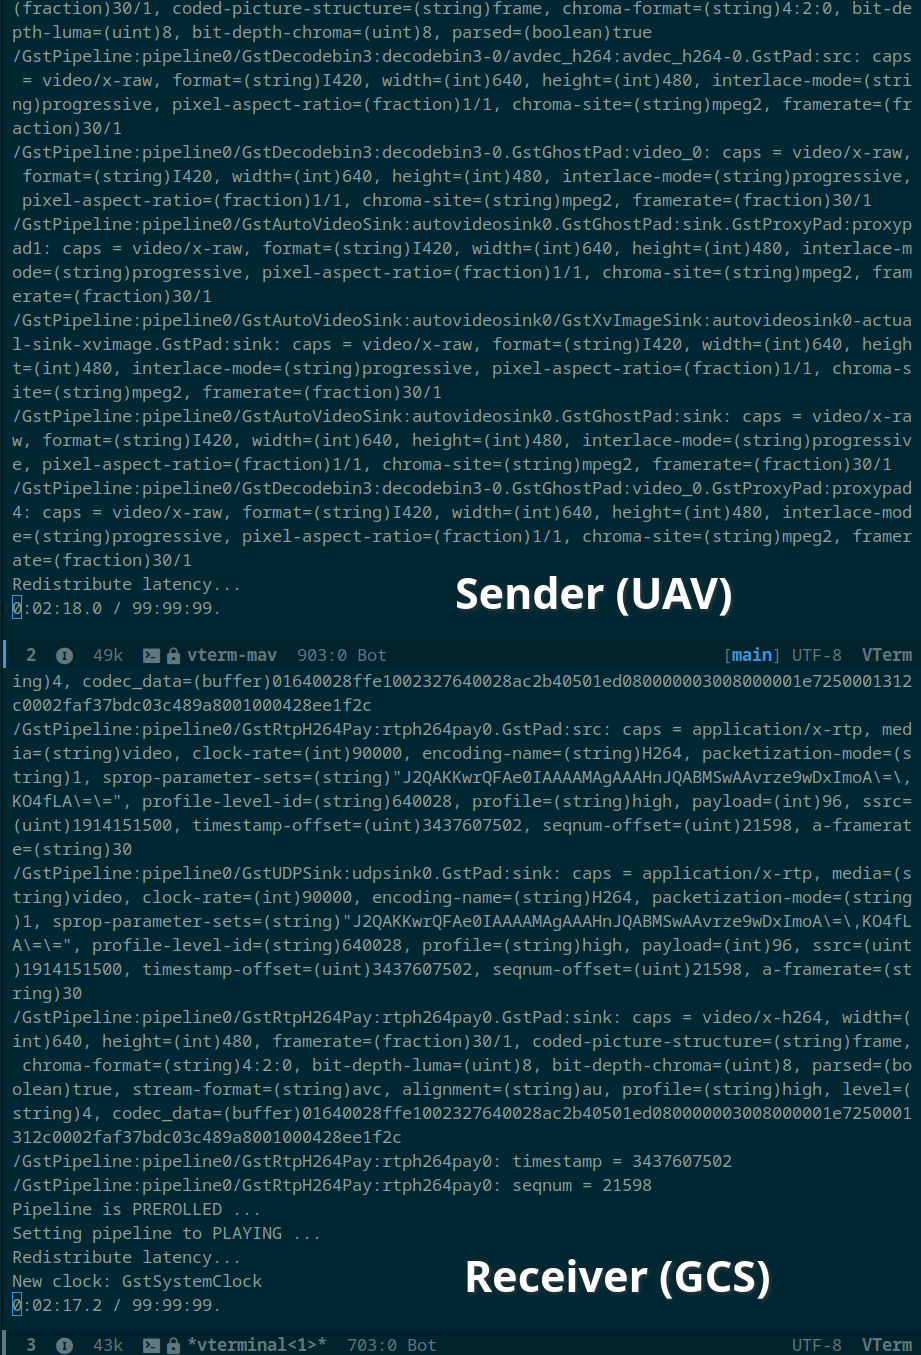
\includegraphics[width=1.0\textwidth]{./img/png/px4-qgc-cam-3}
    \caption{Video pipeline: sender (UAV); receiver (GCS)}%
    \label{fig:px4-qgc-cam-3}
  \end{subfigure}
  \begin{subfigure}[t]{.48\textwidth}
    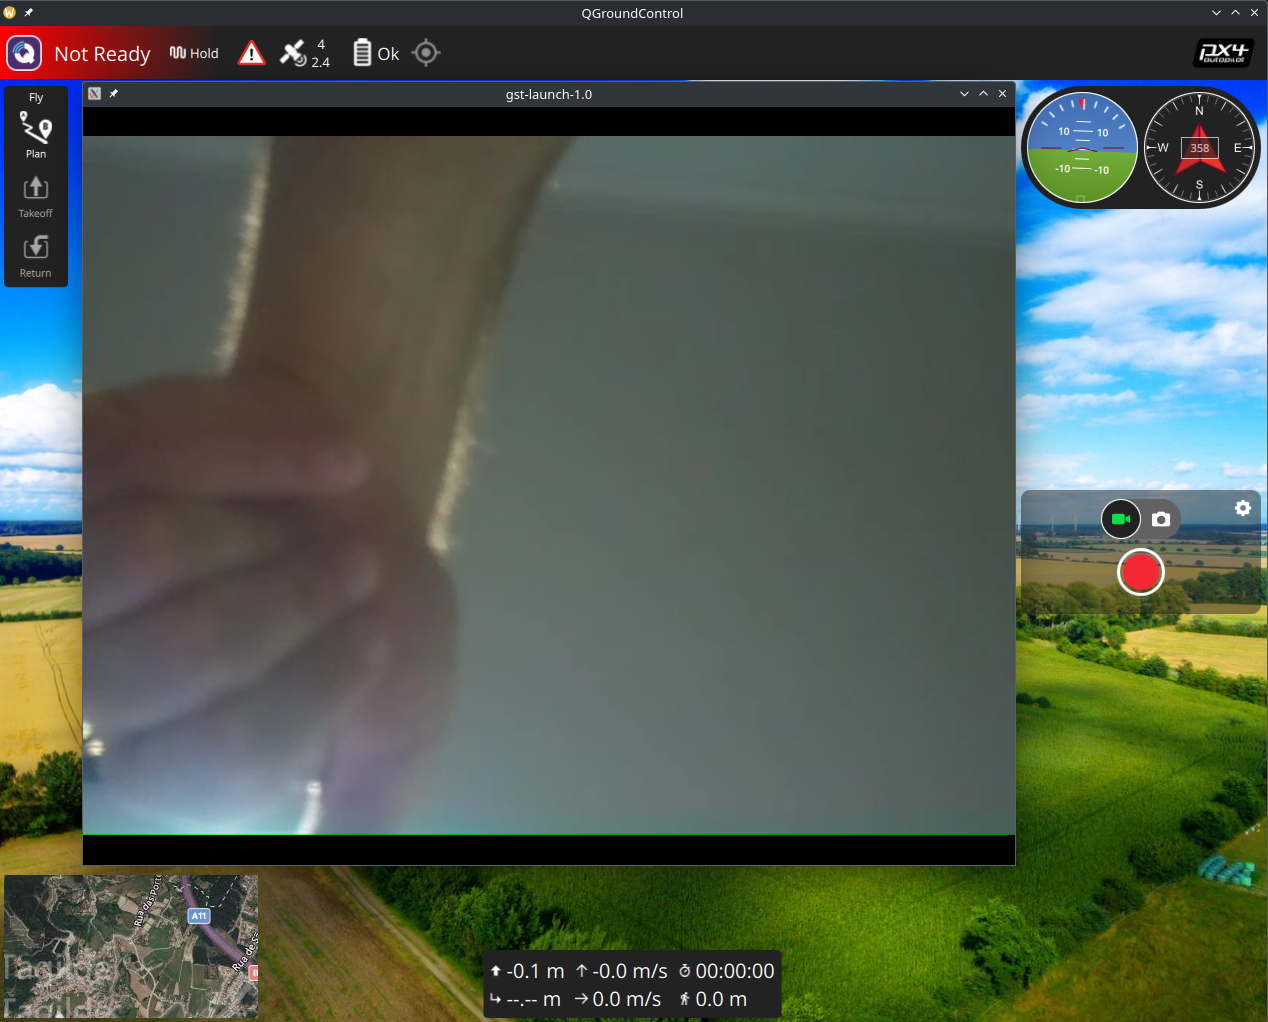
\includegraphics[width=1.0\textwidth]{./img/png/px4-qgc-cam-1}
    \caption{QGroundControl + video receiver}%
    \label{fig:px4-qgc-cam-1}
  \end{subfigure}
  \caption{Video-surveillance pipeline validation}%
  \label{fig:px4-qgc-cam}
\end{figure}

\section{USPFS}
\label{sec:uspfs-implem}
The \gls{uspfs} solution consolidates PX4 and the video-surveillance pipeline on
a custom embedded Linux \gls{os} running on the \gls{uavic}. We first configured
a stable Raspberry~Pi kernel (6.6) with the drivers required by both stacks.
The full configuration is in
\lstinline{configs/uspfs/kernel-uspfs.config}~\cite{thesis-sw-github}. PX4 needs
\gls{spi}/\gls{i2c} (sensors/actuators), \gls{pwm} (motors), and PL011 UART
(\gls{rc}/console). The video pipeline needs V4L2/video and the Mediatek
\lstinline{mt7921au} module for the AX3000 \gls{usb} Wi-Fi dongle.

We then configured Buildroot (\lstinline{configs/uspfs/br-uspfs.config}) to:
(i) integrate the custom kernel; (ii) overlay the PX4 binaries/configuration into
the rootfs; (iii) set the boot console to UART5 (\lstinline{ttyAMA5});
(iv) include \lstinline{GStreamer} for streaming; and (v) package the Mediatek
firmware for the Wi-Fi dongle. This produced the Linux image
\lstinline{Image_1}. Next, we customized the device tree to include the required
hardware (cf.\ Fig.~\ref{fig:hw-map-1}) and combined it with the kernel to form
a self-contained executable blob, \lstinline{linux_1.bin}.

For firmware, we fetched the Raspberry~Pi~4 \gls{bsp} and patched the Arm
Trusted Firmware (\lstinline{bl31.bin}) to redirect the debug console from
UART0 to UART5 (\lstinline{ttyAMA5}). The make fragment
\lstinline{configs/atf/atf-patch.mk}~\cite{thesis-sw-github} shows the inline
\lstinline{serial0}\(\rightarrow\)\lstinline{serial5} change and the UART offset
adjustment. We also customized U-Boot
(\lstinline{configs/uboot/uboot.mk} and \lstinline{configs/uboot/uboot.env}~\cite{thesis-sw-github})
to auto-load \lstinline{linux_1.bin} at the chosen address after
\lstinline{bl31.bin} hands off.

Finally, we wrote the boot artifacts to the SD card: \lstinline{linux_1.bin},
firmware files, secondary bootloaders, and \lstinline{config.txt}. The latter
(\lstinline{configs/uspfs/config.txt}~\cite{thesis-sw-github}) enables early \gls{gic}
interrupts, selects the secondary bootloader and kernel, and sets UART5 as the
system console. We validated boot by monitoring \lstinline{ttyUSB0} at 115200~bps
(\lstinline{screen /dev/ttyUSB0 115200}); the captured log
(\lstinline{logs/boot-uspfs.txt}~\cite{thesis-sw-github}) confirms kernel/Buildroot
versions and UART5 console bring-up. We then repeated the procedures in
Sections~\ref{sec:px4} and~\ref{sec:video-surveillance}, verifying that PX4 and
the streaming pipeline run correctly in the \gls{uspfs} environment.

\section{SSPFS}
\label{sec:sspfs-implem}
For the \gls{sspfs} system we build two isolated Linux guests atop the Bao
hypervisor: one for PX4 and another for the video pipeline. Guest construction
mirrors the \gls{uspfs} flow. For each guest we:
(1) select the kernel, enable the required drivers/packages, and compile a Linux
\gls{os} image (\lstinline{Image_X});
(2) customize the guest-specific device tree;
(3) pack image+\gls{dtb} into a self-contained executable blob
(\lstinline{linux_1.bin} for PX4 and \lstinline{linux_2.bin} for video).

%\subsection{Hypervisor and VM construction}
We forked Bao~\cite{baoRepo-mine} to meet \gls{sspfs}-specific platform needs on
Raspberry~Pi~4, namely redirecting the console from UART0 to UART5 and fixing
its clock/offset. In the platform description
(\lstinline{src/rpi4_desc.c}~\cite{thesis-sw-github}) we set the console base to
\lstinline{0xfe201000} (4~KB-aligned). In the platform header
(\lstinline{src/platform.h}~\cite{thesis-sw-github}) we configured UART5 with a
48~MHz clock and \lstinline{0xa00} offset, yielding the final UART5 address
\lstinline{0xfe201a00}.

The VM layout is specified in
\lstinline{configs/sspfs/bao_sspfs_cfg.c}~\cite{thesis-sw-github}. The PX4
guest receives:
(1) one Arm~A72 core;
(2) two \gls{ram} regions (144~MB and 3~GB) -- the split reserves the first~1~GB
for \gls{dma}-reachable buffers (CMA for \gls{spi}/\gls{i2c} devices);
(3) the essential device set (Fig.~\ref{fig:hw-map-2}).
The Companion guest receives:
(1) three Arm~A72 cores;
(2) two \gls{ram} regions (624~MB and 2~GB), with a large CMA window in the
first~1~GB to sustain the video pipeline;
(3) the \gls{usb} path for camera/Wi-Fi (Fig.~\ref{fig:hw-map-3}).

Shared architectural resources are handled as follows. The architectural timer is
virtualized by Bao and requires no additional work. The firmware mailbox, needed
by devices behind \gls{pcie} (e.g., \gls{usb}), is mediated by the mailbox
supervisor described in Sec.~\ref{sec:superv-mailb-access}: guests bracket
transactions with \lstinline{Start_TX}/\lstinline{End_TX} hypercalls, and Bao
serializes access and routes completions to the correct \gls{vm}.

Finally, we build Bao with the above configuration to produce
\lstinline{bao.bin}, which encapsulates the hypervisor plus both guest blobs.
Boot artifacts (firmware, \lstinline{bl31.bin}, \lstinline{u-boot.bin},
\lstinline{bao.bin}, and \lstinline{config.txt}) are then deployed as in
Sec.~\ref{sec:workflow}, yielding two isolated Linux guests executing under Bao
with the device maps of Fig.~\ref{fig:hw-map-2} and Fig.~\ref{fig:hw-map-3}.

\subsection{Mailbox Supervisor}
The supervision mechanism in Fig.~\ref{fig:design-mailbox} is realized with two pieces:
(1) a mailbox manager inside Bao; and (2) a minimal patch to the Raspberry~Pi
mailbox firmware driver in Linux.
%
Listing~\ref{lst:bao-mailbox-manager} shows the Bao-side manager. We reserve a
dedicated hypercall identifier and two arguments to mark the \emph{start} and
\emph{end} of a mailbox transaction. During platform bring-up,
\lstinline{plat_rpi_init} (invoked before guest boot; see
\lstinline{src/init.c}~\cite{thesis-sw-github}) binds the mailbox’s interrupt to
\lstinline{rpi_mailbox_irq_handler}. When a mailbox event arrives, the handler
injects the configured interrupt ID into the current virtual CPU and suppresses
Bao's default handling path, ensuring completions are delivered to the correct
guest. Guests bracket each transaction with a hypercall
(Listing~\ref{lst:bao-hypercall}), which routes into
\lstinline{rpi_mailbox_hypercall}. On \emph{start}, Bao grants the calling
\lstinline{vCPU} exclusive access to the mailbox (locks and enables the relevant
interrupts); on \emph{end}, it releases the lock and disables the guest’s mailbox
interrupts, allowing the next waiting guest to proceed.

\begin{longlisting}
\centering
\inputminted[]{c}{./listing/rpi_firmware.c}
\caption[SSPFS: mailbox manager added to Bao]{SSPFS: Mailbox manager added to
  Bao (see \lstinline{src/rpi_firmware.c}~\cite{thesis-sw-github})}
\label{lst:bao-mailbox-manager}
\end{longlisting}

\begin{longlisting}
\centering
\inputminted[]{c}{./listing/hypercall.c}
\caption[SSPFS: Bao hypercall manager]{SSPFS: Bao hypercall manager (see
  \lstinline{src/hypercall.c}~\cite{thesis-sw-github})}
\label{lst:bao-hypercall}
\end{longlisting}

On the Linux side (Listing~\ref{lst:linux-rpi-fw}), the mailbox driver uses the
same hypercall identifier and \emph{start}/\emph{end} arguments. After taking its
driver-level lock, it issues an \lstinline{hvc} with the \emph{start} argument
\emph{before} touching the mailbox registers, performs the firmware transaction,
then issues the \emph{end} hypercall and releases the lock. This minimal change
lets Bao serialize mailbox access across guests without altering the driver’s
core logic or firmware protocol.

\begin{longlisting}
\centering
\inputminted[]{c}{./listing/linux-rpi-fw.c}
\caption[SSPFS: Linux's Raspberry Pi mailbox driver — patch]{SSPFS: Linux's
  Raspberry Pi mailbox driver — patch (see \lstinline{src/linux-rpi-fw.c}~\cite{thesis-sw-github})}
\label{lst:linux-rpi-fw}
\end{longlisting}

%%% Local Variables:
%%% mode: LaTeX
%%% TeX-master: "../template"
%%% reftex-default-bibliography: ("../Bibliography/mieeic.bib")
%%% ispell-local-dictionary: "american"
%%% End:
